% !TEX TS-program = knitr
\documentclass[handout]{beamer}\usepackage{graphicx, color}
%% maxwidth is the original width if it is less than linewidth
%% otherwise use linewidth (to make sure the graphics do not exceed the margin)
\makeatletter
\def\maxwidth{ %
  \ifdim\Gin@nat@width>\linewidth
    \linewidth
  \else
    \Gin@nat@width
  \fi
}
\makeatother

\IfFileExists{upquote.sty}{\usepackage{upquote}}{}
\definecolor{fgcolor}{rgb}{0.2, 0.2, 0.2}
\newcommand{\hlnumber}[1]{\textcolor[rgb]{0,0,0}{#1}}%
\newcommand{\hlfunctioncall}[1]{\textcolor[rgb]{0.501960784313725,0,0.329411764705882}{\textbf{#1}}}%
\newcommand{\hlstring}[1]{\textcolor[rgb]{0.6,0.6,1}{#1}}%
\newcommand{\hlkeyword}[1]{\textcolor[rgb]{0,0,0}{\textbf{#1}}}%
\newcommand{\hlargument}[1]{\textcolor[rgb]{0.690196078431373,0.250980392156863,0.0196078431372549}{#1}}%
\newcommand{\hlcomment}[1]{\textcolor[rgb]{0.180392156862745,0.6,0.341176470588235}{#1}}%
\newcommand{\hlroxygencomment}[1]{\textcolor[rgb]{0.43921568627451,0.47843137254902,0.701960784313725}{#1}}%
\newcommand{\hlformalargs}[1]{\textcolor[rgb]{0.690196078431373,0.250980392156863,0.0196078431372549}{#1}}%
\newcommand{\hleqformalargs}[1]{\textcolor[rgb]{0.690196078431373,0.250980392156863,0.0196078431372549}{#1}}%
\newcommand{\hlassignement}[1]{\textcolor[rgb]{0,0,0}{\textbf{#1}}}%
\newcommand{\hlpackage}[1]{\textcolor[rgb]{0.588235294117647,0.709803921568627,0.145098039215686}{#1}}%
\newcommand{\hlslot}[1]{\textit{#1}}%
\newcommand{\hlsymbol}[1]{\textcolor[rgb]{0,0,0}{#1}}%
\newcommand{\hlprompt}[1]{\textcolor[rgb]{0.2,0.2,0.2}{#1}}%

\usepackage{framed}
\makeatletter
\newenvironment{kframe}{%
 \def\at@end@of@kframe{}%
 \ifinner\ifhmode%
  \def\at@end@of@kframe{\end{minipage}}%
  \begin{minipage}{\columnwidth}%
 \fi\fi%
 \def\FrameCommand##1{\hskip\@totalleftmargin \hskip-\fboxsep
 \colorbox{shadecolor}{##1}\hskip-\fboxsep
     % There is no \\@totalrightmargin, so:
     \hskip-\linewidth \hskip-\@totalleftmargin \hskip\columnwidth}%
 \MakeFramed {\advance\hsize-\width
   \@totalleftmargin\z@ \linewidth\hsize
   \@setminipage}}%
 {\par\unskip\endMakeFramed%
 \at@end@of@kframe}
\makeatother

\definecolor{shadecolor}{rgb}{.97, .97, .97}
\definecolor{messagecolor}{rgb}{0, 0, 0}
\definecolor{warningcolor}{rgb}{1, 0, 1}
\definecolor{errorcolor}{rgb}{1, 0, 0}
\newenvironment{knitrout}{}{} % an empty environment to be redefined in TeX

\usepackage{alltt}
\newcommand{\answers}{1}

\usetheme{Marburg}
\setbeamertemplate{navigation symbols}{} 
\setbeamercovered{dynamic}
\setbeamertemplate{footline}
{
  \leavevmode%
  \hbox{%
  \begin{beamercolorbox}[wd=.333333\paperwidth,ht=2.25ex,dp=1ex,center]{author in head/foot}%
    \usebeamerfont{author in head/foot}\copyright $\ $ \insertshortauthor%~~\beamer@ifempty{\insertshortinstitute}{}{(\insertshortinstitute)}
  \end{beamercolorbox}%
  \begin{beamercolorbox}[wd=.333333\paperwidth,ht=2.25ex,dp=1ex,center]{title in head/foot}%
    \usebeamerfont{title in head/foot} \insertinstitute
  \end{beamercolorbox}%
  \begin{beamercolorbox}[wd=.333333\paperwidth,ht=2.25ex,dp=1ex,right]{date in head/foot}%
    \usebeamerfont{date in head/foot}\insertshortdate{}\hspace*{2em}
    \insertframenumber{} / \inserttotalframenumber\hspace*{2ex} 
  \end{beamercolorbox}}%
  \vskip0pt%
}

\usepackage{amsmath}
\usepackage{caption}
\usepackage{color}
\usepackage{enumerate}
\usepackage{listings}
\usepackage{hyperref}
\usepackage{mathrsfs}
\usepackage{natbib}
\usepackage{url}

\providecommand{\all}{\ \forall \ }
\providecommand{\bs}{\backslash}
\providecommand{\e}{\varepsilon}
\providecommand{\E}{\ \exists \ }
\providecommand{\lm}[2]{\lim_{#1 \rightarrow #2}}
\providecommand{\m}[1]{\mathbb{#1}}
\providecommand{\nv}{{}^{-1}}
\providecommand{\ov}[1]{\overline{#1}}
\providecommand{\p}{\newpage}
\providecommand{\q}{$\quad$ \newline}
\providecommand{\rt}{\rightarrow}
\providecommand{\Rt}{\Rightarrow}
\providecommand{\vc}[1]{\boldsymbol{#1}}
\providecommand{\wh}[1]{\widehat{#1}}

\hypersetup{colorlinks,linkcolor=,urlcolor=blue}
\numberwithin{equation}{section}

\definecolor{dkgreen}{rgb}{0,0.6,0}
\definecolor{gray}{rgb}{0.5,0.5,0.5}
\definecolor{mauve}{rgb}{0.58,0,0.82}

\lstset{ 
  language=C,                % the language of the code
  basicstyle= \footnotesize,           % the size of the fonts that are used for the code
  numberstyle= \tiny \color{white},  % the style that is used for the line-numbers
  stepnumber=2,                   % the step between two line-numbers. 
  numbersep=5pt,                  % how far the line-numbers are from the code
  backgroundcolor=\color{white},      % choose the background color. You must add \usepackage{color}
  showspaces=false,               % show spaces adding particular underscores
  showstringspaces=false,         % underline spaces within strings
  showtabs=false,                 % show tabs within strings adding particular underscores
  frame=lrb,                   % adds a frame around the code
  rulecolor=\color{black},        % if not set, the frame-color may be changed on line-breaks within not-black text 
  tabsize=2,                      % sets default tabsize to 2 spaces
  captionpos=t,                   % sets the caption-position 
  breaklines=true,                % sets automatic line breaking
  breakatwhitespace=false,        % sets if automatic breaks should only happen at whitespace
  %title=\lstname,                   % show the filename of files included with \lstinputlisting;
  keywordstyle=\color{blue},          % keyword style
  commentstyle=\color{gray},       % comment style
  stringstyle=\color{dkgreen},         % string literal style
  escapeinside={\%*}{*)},            % if you want to add LaTeX within your code
  morekeywords={*, ...},               % if you want to add more keywords to the set
  xleftmargin=0.053in, % left horizontal offset of caption box
  xrightmargin=-.03in % right horizontal offset of caption box
}

%\DeclareCaptionFont{white}{\color{white}}
%\DeclareCaptionFormat{listing}{\parbox{\textwidth}{\colorbox{gray}{\parbox{\textwidth}{#1#2#3}}\vskip-0.05in}}
%\captionsetup[lstlisting]{format = listing, labelfont = white, textfont = white}
%For caption-free listings, comment out the 3 lines above and uncomment the 2 lines below.
 \captionsetup{labelformat = empty, labelsep = none}
 \lstset{frame = single}





\title{The Design of Statistical Studies (Ch 1-2)}
\author{Will Landau}
\date{January 22, 2013}
\institute{Iowa State University}

\begin{document}

\begin{frame}
\titlepage
 \end{frame}
 
 \AtBeginSection[]
{
   \begin{frame}
       \frametitle{Outline}
       \tableofcontents[currentsection]
   \end{frame}
}

\section{Common Experimental Designs}

\subsection{Completely Randomized Design}


\begin{frame}
\frametitle{Completely Randomized Design} \small

\begin{itemize}
\item {\bf Completely Randomized Design} 
\begin{itemize}
\pause \item an experimental design with one treatment variable and no blocking variables.
\pause \item Sample units are randomly assigned to treatment levels.
\end{itemize} 
\pause \item Example: metallurgy
\begin{itemize}
 \item Test the effect of different additives on the corrosion rate of steel. 
\pause \item Sample: 12 pieces of raw iron
\pause \item Treatment: additive (A, B, or C).
\pause \item Treatment groups: A (units 1-4), B (units 5-8), and C (units 9-12)
\end{itemize} 
\end{itemize}
\scriptsize
\begin{center}
\begin{tabular}{c|c}
Sample unit & Additive \\ \hline
1 & A \\ 
2 & A \\ 
3 & A \\ 
4 & A \\ 
5 & B \\ 
6 & B \\ 
\end{tabular} $\quad$ \begin{tabular}{c|c}
Sample unit & Additive \\ \hline
7 & B \\ 
8 & B \\ 
9 & C \\ 
10 & C \\ 
11 & C \\ 
12 & C \\ 
\end{tabular}
\end{center}
\end{frame}

\subsection{Factorial Design}


\begin{frame}
\frametitle{Factorial Design} \small

\begin{itemize}
\item {\bf Factorial Design} 
\begin{itemize}
\pause \item an experimental design with multiple treatment variable (as factors) and no blocking variables.
\pause \item Each sample unit is randomly assigned to a combination of treatment levels.
\end{itemize} 
\pause \item Example: metallurgy: a $3 \times 2$ factorial version
\begin{itemize}
\pause \item Treatment 1: additive (A, B, or C).
\pause \item Treatment 2: temperature (high or low)
\pause \item Treatment groups: A high (units 1-2), A low (units 3-4), B high (units 5-6), B low (units 7-8), C high (units 9-10), C low (units 11-12), 
\end{itemize} 
\end{itemize}
\scriptsize
\begin{center}
\begin{tabular}{c|c|c}
Unit & Additive & Temp \\ \hline
1 & A & high \\ 
2 & A & high \\ 
3 & A & low \\ 
4 & A & low \\ 
5 & B & high \\ 
6 & B & high\\ 
\end{tabular}$\quad$ \begin{tabular}{c|c|c}
Unit & Additive & Temp \\ \hline
7 & B & low \\ 
8 & B & low \\ 
9 & C & high \\ 
10 & C & high \\ 
11 & C & low \\ 
12 & C & low \\ 
\end{tabular}
\end{center}
\end{frame}


\begin{frame}
\frametitle{Metallurgy example: a $2^3$ factorial version} \scriptsize

\begin{itemize}
 \item Sample: 16 pieces of iron.
\pause \item Treatments:
\begin{itemize}
 \item Treatment 1: additive (A or B)
\pause \item Treatment 2: temperature (high or low)
\pause \item Treatment 3: smelting time (long or short)
\end{itemize}
\pause \item Treatment groups: A high long (units 1-2) A high short (units 3-4), $\ldots$, B low short (units 11-12).
\end{itemize}

\begin{center}
\begin{tabular}{c|c|c|c}
Unit & Add & Temp & Smelt \\ \hline
1 & A & high & long \\ 
2 & A & high & long \\ 
3 & A & high & short \\ 
4 & A & high & short \\ 
5 & A & low & long \\ 
6 & A & low & long\\ 
7 & A & low & short \\ 
8 & A & low & short \\ 
\end{tabular}$\quad$ \begin{tabular}{c|c|c|c}
Unit & Add & Temp & Smelt \\ \hline
9 & B & high & long \\ 
10 & B & high & long \\ 
11 & B & high & short \\ 
12 & B & high & short \\ 
13 & B & low & long \\ 
14 & B & low & long \\ 
15 & B & low & short \\ 
16 & B & low & short \\ 
\end{tabular}
\end{center}
\end{frame}


\subsection{Randomized Complete Block Design}


\begin{frame}
\frametitle{Randomized Complete Block Design} \small

\begin{itemize}
\item {\bf Randomized Complete Block Design} 
\begin{itemize}
\pause \item an experimental design with one or more treatment variable and at least one blocking variable.
\pause \item Within each block separately, sample units are assigned to treatment groups 
\end{itemize} 
\pause \item Example: metallurgy
\begin{itemize}
\item Treatment: additive (A, B, or C).
\pause \item Blocking variable: pig iron supplier (Amset or Miller and Co.)
\end{itemize} 
\end{itemize}
\scriptsize
\begin{center}
\begin{tabular}{c|c|c}
Unit & Supplier & Add\\ \hline
1 & Amset & A \\ 
2 & Amset & A \\ 
3 & Amset & B \\ 
4 & Amset & B \\ 
5 & Amset & C \\
6 & Amset & C \\
\end{tabular} $\quad$ \begin{tabular}{c|c|c}
Unit & Supplier & Add \\ \hline
7 & Miller & A \\ 
8 & Miller & A \\ 
9 & Miller & B \\ 
10 & Miller & B \\ 
11 & Miller & C \\ 
12 & Miller & C \\ 
\end{tabular}
\end{center}
\end{frame}


\section{Simple Random Sampling}


\begin{frame}
\frametitle{Simple Random Sampling}
\begin{itemize}
\item {\bf Simple Random Sampling}: drawing a sample of $n$ units from a finite population of $N$ units such that every possible $n$-sized subset of the population has an equal chance of being selected.
\pause \item Use either a computerized random number generator or a \href{http://will-landau.com/stat305/tables/random-digits.pdf}{table of random digits}.
\end{itemize}

\begin{center}
\setkeys{Gin}{width=1\textwidth} 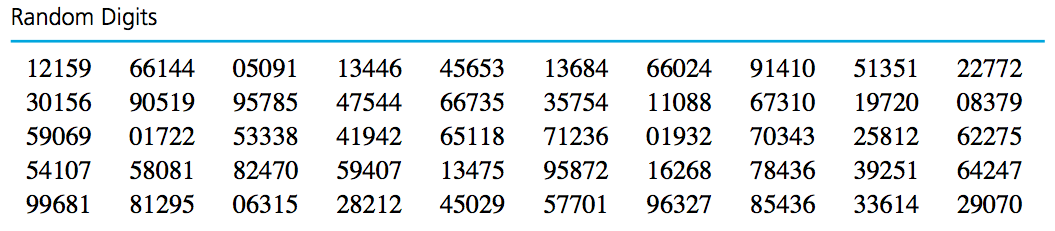
\includegraphics{../../fig/rdigits.png}
\end{center}

\end{frame}


\begin{frame}
\frametitle{Steps of Simple Random Sampling} \small

\begin{enumerate}[1. ]
\item Let $M$ be the number of digits in the number $N -1$, where $N$ is the population size. (If $N = 1000$ then $M = 3$ digits.)
\pause \item Give each member of the population an $M$-digit index, $i$ (say, $i = 000, 001, \ldots, 999$)
\pause \item Move through the table of random digits from left to right, top to bottom, selecting population members for the sample when you encounter their indices (ignoring indices that have already been chosen) until you have selected $n$ units for the sample.
\end{enumerate}

\begin{center}
\setkeys{Gin}{width=1\textwidth} 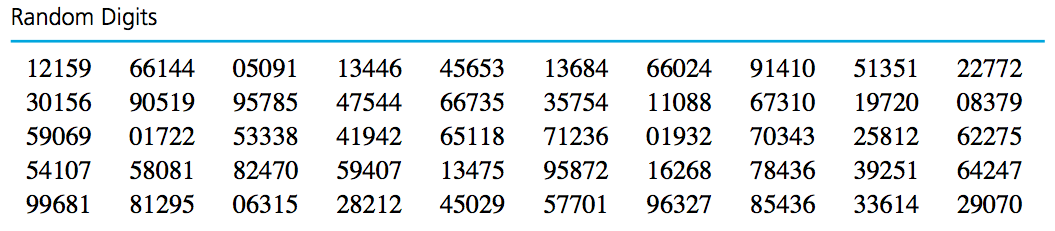
\includegraphics{../../fig/rdigits.png}
\end{center}
\end{frame}

\begin{frame}
\frametitle{Your turn: metallurgy}

Using the table of random digits below, take a simple random sample of 12 units of pig iron out of a shipment of 90 units.

\begin{center}
\setkeys{Gin}{width=1\textwidth} 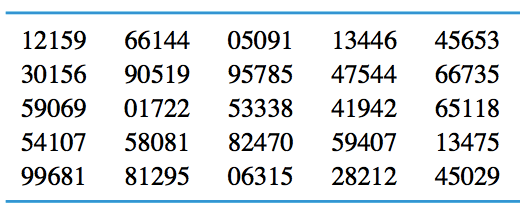
\includegraphics{../../fig/rdigitsshort.png}
\end{center}

\end{frame}


\begin{frame}<handout:\answers>
\frametitle{Your turn: metallurgy}

Solution:
\begin{itemize}
\item Indexed the members of the population from 00 to 89.
\pause \item Selected units 12, 15, 61, 44, 5, 9, 11, 34, 46, 45, 65, and 33 for the sample.
\end{itemize}

\begin{center}
\setkeys{Gin}{width=1\textwidth} 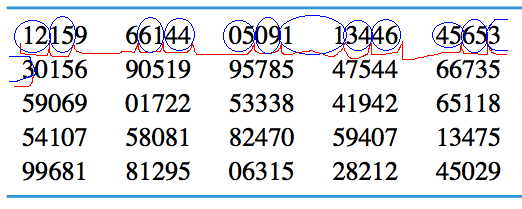
\includegraphics{../../fig/rdigitsshortmarked.png}
\end{center}

\end{frame}



\section{Randomization}

\subsection{Randomization without blocks}


\begin{frame}
\frametitle{Randomization}

\begin{itemize}
\item {\bf Randomization}: assigning sample units to treatment groups in an experiment such that every set of assignments is equally likely.
\pause \item Steps to randomize $n$ sample units to $t$ treatment groups, each of size $s$ ($n = ts$):
\begin{enumerate}[1. ]
\pause \item Use the table of random digits to select $s$ units for treatment group 1 from the experimental sample of $n$ units.
\pause \item Continuing from your last spot in the table, select $s$ units for treatment group 2 from the remaining $n - s$ units in the experimental sample.
\pause \item Continue this process until you have selected $t - 1$ treatment groups. The remaining units will belong to the last treatment group.
\end{enumerate}
\end{itemize}
\end{frame}


\begin{frame}
\frametitle{Your turn: metallurgy}

Randomize our experimental sample of 12 units of pig iron to thee treatment groups (for additives A, B, and C).

\begin{center}
\setkeys{Gin}{width=1\textwidth} 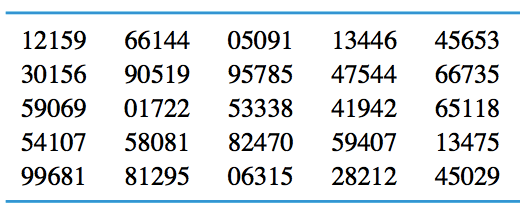
\includegraphics{../../fig/rdigitsshort.png}
\end{center}

\end{frame}

\begin{frame}<handout:\answers>
\frametitle{Your turn: metallurgy}

Solution:
\begin{itemize}
\item Units 05, 09, 11, and 01 for group A (blue).
\pause \item Units 06, 07, 08, and 02 for group B (green).
\pause \item Units 03, 04, 10, and 00 for group C (leftover).
\end{itemize}


\begin{center}
\setkeys{Gin}{width=1\textwidth} 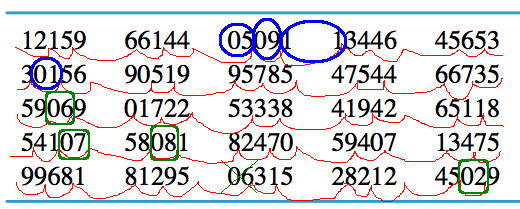
\includegraphics{../../fig/rdigitsshortranomize1.png}
\end{center}

\end{frame}



\begin{frame}
\frametitle{For randomization in factorial studies, know your treatment groups.}


\begin{itemize}
\item Example: metallurgy: a $3 \times 2$ factorial version
\begin{itemize}
\pause \item Sample: $n = 12$ units
\pause \item Treatment 1: additive (A, B, or C).
\pause \item Treatment 2: temperature (high or low).
\end{itemize} 
\end{itemize}

\begin{enumerate}[1. ]
\pause \item How many treatment groups do we have?
\pause \item How many units of the experimental sample should I randomize to each treatment group?
\end{enumerate}

\end{frame}


\begin{frame}<handout:\answers>
\frametitle{Know you treatment groups: answers}

\begin{enumerate}[1. ]
\item $3 \times 2 = 6$ treatment groups.
\pause \item Each treatment group has $12 / 6 = 2$ units of pig iron.
\end{enumerate}

\end{frame}


\subsection{Randomization with Blocks}

\begin{frame}
\frametitle{Randomization with blocks}
\small
\begin{itemize}
\item Randomize units to treatments \emph{within each block}. \q

\begin{tabular}{c|c|c}
Unit & Supplier & Add\\ \hline
1 & Amset & A \\ 
2 & Amset & A \\ 
3 & Amset & B \\ 
4 & Amset & B \\ 
5 & Amset & C \\
6 & Amset & C \\
\end{tabular} $\quad$ \begin{tabular}{c|c|c}
Unit & Supplier & Add \\ \hline
7 & Miller & A \\ 
8 & Miller & A\\ 
9 & Miller & B \\ 
10 & Miller & B \\ 
11 & Miller & C \\ 
12 & Miller & C \\ 
\end{tabular} \q

\pause \item For the metallurgy block design:

\begin{itemize}
\item Randomize all \emph{Amset units} to treatments A, B, and C
\pause \item Then, picking up where you left off in the  table of random digits,
randomize all \emph{Miller units} to treatments A, B, and C.
\end{itemize}
\end{itemize}


\end{frame}

\begin{frame}
\frametitle{Your turn: metallurgy block design}

\begin{itemize}
\item Given:
\begin{itemize}
\item 2 blocks (Amset and Miller).
\item 3 treatment levels (A, B, and C).
\end{itemize}
\item Randomize the 12 units of pig iron to treatment groups
\end{itemize}

\begin{center}
\setkeys{Gin}{width=1\textwidth} 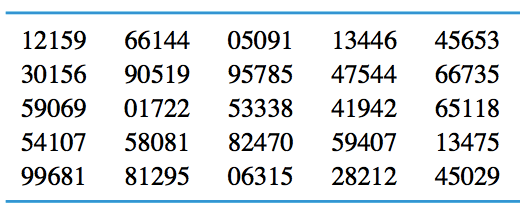
\includegraphics{../../fig/rdigitsshort.png}
\end{center}
\end{frame}


\begin{frame}<handout:\answers>
\frametitle{The Amset Block}

\begin{itemize}
 \item Index the 6 Amset units of pig iron from 0 to 5.
\pause \item Using the table of random digits, select:
\begin{itemize}
\pause \item Units 1 and 2 for group A (blue).
\pause \item Units 5 and 4 for group B (green).
\pause \item Units 0 and 3 for group C (leftover).
\end{itemize}
\end{itemize}

\begin{center}
\setkeys{Gin}{width=1\textwidth} 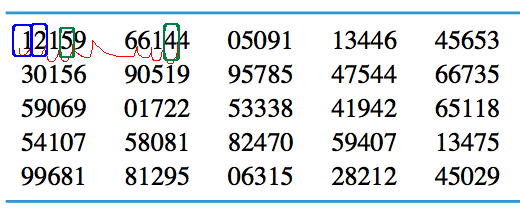
\includegraphics{../../fig/rdigitsshortAmset.png}
\end{center}

\end{frame}


\begin{frame}<handout:\answers>
\frametitle{The Miller Block}

\begin{itemize}
 \item Index the 6 Miller units of pig iron from 0 to 5.
\pause \item Using the table of random digits, select:
\begin{itemize}
\pause \item Units 4 and 0 for group A (orange).
\pause \item Units 5 and 1 for group B (red).
\pause \item Units 2 and 3 for group C (leftover).
\end{itemize}
\end{itemize}
\begin{center}
\setkeys{Gin}{width=1\textwidth} 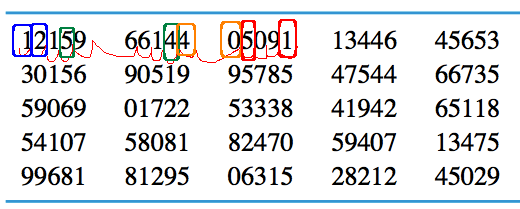
\includegraphics{../../fig/rdigitsshortMiller.png}
\end{center}
\end{frame}


%\begin{frame}
%\frametitle{Sources}
%\begin{enumerate}[1. ]
%\item Some source
%\end{enumerate}
%\end{frame}

\end{document}
